\documentclass[11pt,letterpaper]{article}

%% === margins ===
%\addtolength{\hoffset}{-0.75in} \addtolength{\voffset}{-0.75in}
%\addtolength{\textwidth}{1.5in} \addtolength{\textheight}{1.6in}
%% === basic packages ===
\usepackage{latexsym}
\usepackage{amssymb,amsmath}
\usepackage{graphicx}
\usepackage{verbatim}
\usepackage{ccaption}
\usepackage{booktabs}
%% === bibliography packages ===
\usepackage{natbib}
\bibliographystyle{asa}
%% === hyperref options ===
\usepackage{color}
\usepackage[table]{xcolor}
\usepackage{graphicx} 
\usepackage{booktabs} 
\usepackage{xcolor}
\usepackage{colortbl}
\usepackage{multirow}
\usepackage{amsmath}
\usepackage{rotating}
\usepackage{lscape}
\usepackage{longtable}
\usepackage{subfig}
\usepackage[pdftex, bookmarksopen=true, bookmarksnumbered=true, 
pdfstartview=FitH, breaklinks=true, urlbordercolor={1 1 1}, citebordercolor={1 1 1}]{hyperref}  
\usepackage{lipsum} %package to eliminate pagenumbering, using \pagenumbering{gobble}
% === dcolumn package ===
\usepackage{dcolumn}
\newcolumntype{.}{D{.}{.}{-1}}
\newcolumntype{d}[1]{D{.}{.}{#1}}
% === theorem package ===
\usepackage{theorem}
\theoremstyle{plain}
\theoremheaderfont{\scshape}
\newtheorem{proposition}{Proposition}
\newtheorem{assumption}{Assumption}
\def\qed{\hfill \vrule height7.5pt width6.17pt depth0pt}

\renewcommand{\arraystretch}{1.2}
\newcolumntype{R}[1]{>{\currentrowstyle\raggedleft\arraybackslash}p{#1}}

% ==== rotating package ===
\usepackage{rotating}

% ==== threeparttable package ===
\usepackage[para]{threeparttable}

% == spacing between sections and subsections
\usepackage[compact]{titlesec} 

\newtheorem{theorem}{Theorem}
%\newtheorem{proposition}[theorem]{Proposition}
\newtheorem{corollary}[theorem]{Corollary}
\newtheorem{lemma}[theorem]{Lemma}
\newtheorem{definition}{Definition}
\theoremstyle{remark}
\newtheorem{rem}{Remark}

\newcommand{\itl}{\textit}
\newcommand{\beg}{\begin}
\newcommand{\tbf}{\textbf}
\newcommand{\non}{\nonumber}
\newcommand{\noi}{\noindent}
\newcommand{\bs}{\bigskip}
\newcommand{\tcr}[1]{\textcolor{red}{#1}}
\newcommand{\tcb}[1]{\textcolor{blue}{#1}}
\newcommand{\hlight}[1]{\colorbox{yellow}{#1}}
\newcommand{\ds}{\displaystyle}
\definecolor{Gray}{gray}{0.9}

\textwidth=16cm \textheight=23cm
%\parskip=\medskipamount
\parindent=0.3in
\topmargin=-2cm \oddsidemargin=0cm

\numberwithin{equation}{section}

\begin{document}

\newcommand\spacingset[1]{\renewcommand{\baselinestretch}%
{#1}\small\normalsize}
\spacingset{1}

\newcommand{\blind}{0} \newcommand{\tit}{Supplementary Materials for ``Quantifying the Contribution of Earlier Detection and Advancements in Treatment on Gains in Life Expectancy for US Breast Cancer Patients Since 1975''}
%%%%%%%%%%%%%%%%%%%%%%%%%%%%%%%%%%%%%%%%%%%%%%%%%%%%%%%%%%%%%%%%%%%%%%%%

\if0\blind

 {\title{\bf \tit}
 
  \author{Samir Soneji\thanks{Norris Cotton Cancer Center and
      Dartmouth Institute for Health Policy \& Clinical Practice,
      Geisel School of Medicine at Dartmouth. Email: \href{mailto:samir.soneji@dartmouth.edu}{samir.soneji@dartmouth.edu}}
  \quad \quad 
  Hiram Beltr\'{a}n-S\'{a}nchez\thanks{Community Health Sciences, University of California, Los Angeles. Email:
    \href{mailto:beltrans@ucla.edu}{beltrans@ucla.edu}}}

\date{ }

\maketitle} \fi

% \begin{abstract}
% {\textbf{Background}.  US breast cancer mortality rates declined by 32\% since 1975, although the precise contributions of earlier detection and advancements in breast cancer treatment remain unknown.  We quantify the contributions of these two factors, as well as advancements in the treatment of other diseases, on gains in life expectancy among breast cancer patients.

% \textbf{Methods}.  We obtained annual incidence-based case fatality rates for 664,000 breast cancer patients aged 40 years and older from the Surveillance, Epidemiology, and End Results registries, 1975 to 2012.  We used life-table methods to calculate the gain in life expectancy and quantify the three constituent components of this gain: [1] earlier detection, [2] advancements in breast cancer treatment, and [3] advancements in the treatment of other diseases.  We additionally quantify which age groups contributed the most to the overall contribution of earlier detection.  We assumed a 10\% overdiagnosis level for tumors $\leq$3cm, and varied the level up to 32\% in a sensitivity analysis.

% \textbf{Results}.  Overall,  life expectancy increased 10.94 years between 1975 and 2002 for a 40-year old newly diagnosed breast cancer patient.  Advancements in breast cancer treatment contributed more to the gain in life expectancy than earlier detection: 6.79 years (62\%) versus 2.92 years (27\%).  Advancements in the treatment of other diseases contributed the remaining 1.25 years to this gain (11\%).  By age group, earlier detection among 40-49 year olds contributed more to the overall contribution of earlier detection (0.56 years) than 50-59 and 60-69 year olds (0.45 and 0.41 years, respectively).  We reached nearly identical substantive conclusions varying the level of overdiagnosis.

% \textbf{Conclusion}.  Life expectancy among breast cancer patients increased over time primarily because of advancements in breast cancer treatment, although the contribution of earlier detection was not trivial.}
% \end{abstract}
\if1\blind \title{\bf \tit} \maketitle \fi

\pdfbookmark[1]{Title Page}{Title Page}

\thispagestyle{empty}
\setcounter{page}{0}



\newpage
\clearpage
%%%%%%%%%%%%%%%%%%%%%%%%%%%%%%%%%%%%%%%%%%%%%%%%%%%%%%%%%%%%%%%%%%%%%%
 \setcounter{table}{0}  % reset counter for equation numbers
 \setcounter{figure}{0}  % reset counter for equation numbers
 \setcounter{page}{1}
 \renewcommand{\figurename}{Supplemental Figure}
 \renewcommand{\tablename}{Supplemental Table}
%\clearpage
%\pagenumbering{gobble}
\appendix

\spacingset{1.5}
\section{Computation of Incidence-Based Case Fatality Rates}
An incidence-based case fatality rate for a specific cohort of newly
diagnosed breast cancer patients equals the ratio of [1] the number of
deaths occurring for this cohort up to 10 years beyond their diagnosis
and [2] the total number of person-years lived by this cohort up to 10
years beyond their diagnosis.  For example, 556 women aged 65-69 years
were diagnosed with $<$1 cm breast cancer in 2001.  Between 2001 and
2011, 22 of these women died of breast cancer and another 107 died of
a competing cause of death.  This entire cohort lived a total of
5099.5 person-years over the 10-year period.  Thus, the
incidence-based case fatality rate from breast cancer equaled
22/5099.5 and the incidence-based case fatality rate from competing
causes of death equaled 107/5099.5.  Also, the proportion of women
diagnosed with <1cm breast cancer in 2001 equaled 4,602 out of 19,029
newly diagnosed breast cancers (24.2\%).

\section{Adjustment for Overdiagnosis}
Suppose 10\% of the 556 women aged 65-69 years old diagnosed with $<1$cm
breast cancer in 2001 were overdiagnosed, the observed case fatality
rate from breast cancer (22/5099.5) would become 22/[5099.5 -
0.10*5099.5].  Formally, let $\mathcal{A}$ be a set of starting ages
for age intervals analyzed (e.g., 40, 45, \dots, $\omega=100$ years), $\mathcal{T}$ be a set of
years (e.g., 1975, \dots 2002), and $\mathcal{S}$ be a set of tumor
sizes at diagnosis (e.g., $<1$ cm, 1-2 cm, 2-3 cm, 3-5 cm, and 5+ cm).
Let $\alpha_s$ represent the assummed level of overdiagnosis for tumor
size $s\in\mathcal{S}$.  Let $m_{a,t,s}$ represent the observed case
fatality rate for age group $a \in \mathcal{A}$, year $t \in
\mathcal{T}$, and tumor size $s \in \mathcal{S}$.  Then, the case
fatality rate adjusted for overdiagnosis, $m^*_{a,t,s}$, equals,
$\frac{1}{1-\alpha_s} \times m_{a,t,s}$.

\section{Computation of Tumor Size-Specific Life Expectancy}
The life expectancy of a breast cancer patient newly diagnosed at age
$a^*\in\mathcal{A}$, at time $t$, and with tumor size $s$ equals:
\begin{eqnarray}
 e_s(a^*,t)=\int_{a^*}^{\omega} e^{\left( -\int_{a*}^{a}\mu_s(y,t)\,dy \right)}da =\int_{a^*}^{\omega} e^{\left(-\sum_{a=a*}^{a}n\,m^*_{a,t,s}\right)}\,da ,
\end{eqnarray} 
where $\mu_s(a,t)$ and $m^*_{a,t,s}$ represent the hazard of mortality
and case fatality rate adjusted for overdiagnosis, respectively; $n$
is the width of the age interval; and $\omega$ is the starting age of
the final and open-ended age interval.

\section{Schematic Representation of the Methodology}
For simplicity, consider three mutually exclusive and exhaustive
categories of tumor size: 1, 2, and 3 (e.g., $<$1cm, 1-2cm, and
$\geq$2cm).  Suppose the distribution of tumor size at cancer
diagnosis remained constant between times 1 and 2 (Supplemental
Figure~\ref{fig:simple_case}, Panel A), tumor size-specific case
fatality rates from breast cancer decreased between times 1 and 2
(Supplemental Figure~\ref{fig:simple_case}, Panel B), and tumor
size-specific case fatality rates from competing causes of death
remained constant between times 1 and 2 (Supplemental
Figure~\ref{fig:simple_case}, Panel B).  Tumor size-specific life
expectancy increased between times 1 and 2 because tumor size-specific
case fatality rates from breast cancer decreased over the time period
(Supplemental Figure~\ref{fig:simple_case}, Panel C).  Overall life
expectancy at each time equals the weighted average of tumor
size-specific life expectancy, where the weights equal the
distribution of tumor sizes at cancer diagnosis at times 1 and 2,
respectively.  Overall life expectancy grew between times 1 and 2, and
this gain was entirely due to decreases in tumor size-specific case
fatality rates from breast cancer (Supplemental
Figure~\ref{fig:simple_case}, Panel D).  In actuality, all three
aforementioned factors change over time and contribute to the gain in
life expectancy.  We quantify the individual contribution of each of
these three constituent components.  We also utilize the same
demographic method to further disaggregate these three contributions
by age group in Section~\ref{sec:age}.
\begin{figure}[h]
\begin{center}
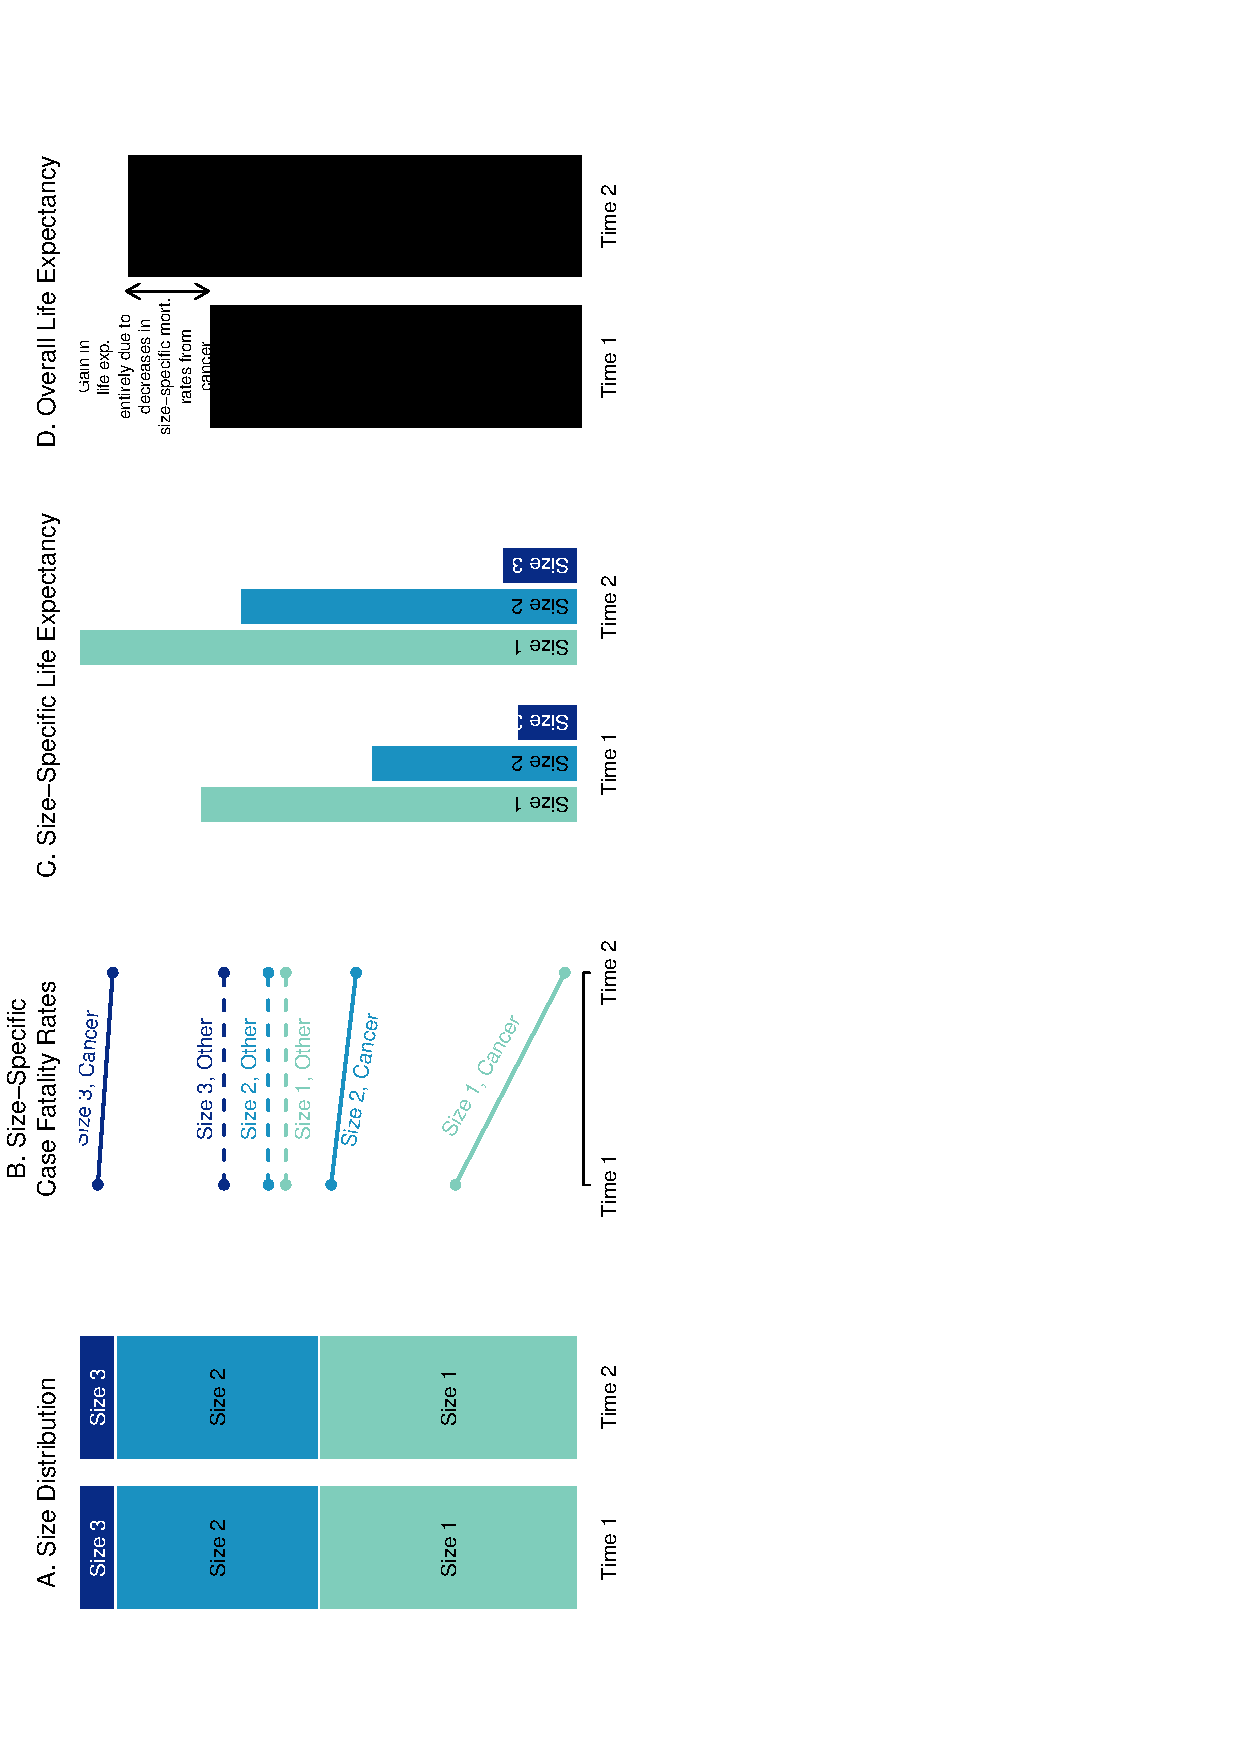
\includegraphics[trim=0 220 0 0,clip,width=\linewidth]{appendix_figure1}
\spacingset{1}\caption{The gain in life expectancy depends
  on three factors: (A) changes in the tumor size distribution at
  cancer diagnosis, (B) changes in tumor size-specific case fatality rates from
  breast cancer, and (C) changes in tumor size-specific case fatality rates from
  competing causes of death.}
\label{fig:simple_case}
\end{center}
\end{figure}

\section{Decomposition by Tumor Size and Case Fatality Rates from
  Breast Cancer and Other Causes of Death}
Let $\pi_s(t)$ equal the proportion of breast cancer patients
diagnosed with tumor size $s$ in year $t$.  Let $e_s(a,t)$ equal the
tumor size-specific life expectancy at age $a$. The overall life
expectancy at age $a$ and time $t$, $e(a,t)$, equals:
\begin{eqnarray}
  e(a,t)=\sum_{s\in\mathcal{S}}\,\pi_s(t)\,e_s(a,t), \notag
\end{eqnarray}
where $\sum_{s\in\mathcal{S}}\,\pi_s=1$. 

The change in life expectancy at age $a$ between times $t_1$ and $t_2$
can be decomposed using the methodology of \cite{Kitagawa55}:
\begin{align}
  e(a,t_2)-e(a,t_1)&=\sum_{s\in\mathcal{S}}\left[\,\pi_s(t_2)\,e_s(a,t_2)- \pi_s(t_1)\,e_s(a,t_1)\right]  \notag\\
  \hspace{-0.7in} &=\sum_{s\in\mathcal{S}}\left[\pi_s(t_2)-\pi_s(t_1)
  \right]\left[\frac{e_s(a,t_1)+e_s(a,t_2)}{2}\right]+ \notag\\
  &\phantom{=}\sum_{s\in\mathcal{S}}\left[e_s(a,t_2)-e_s(a,t_1)
  \right]\left[\frac{\pi_s(t_1)+\pi_s(t_2)}{2}\right].
 \label{eqn:decomp.basic}
\end{align}
 
Equation~\ref{eqn:decomp.basic} quantifies how much of the change in life
expectancy at age $a$ between times $t_1$ and $t_2$ is due to: [a]
shifts in the share of cancer tumor size (first term) and [b] changes
in tumor-size-specific life expectancy (second term).

We can further decompose the second term of
equation~\ref{eqn:decomp.basic} by cause of death. In doing so, we can
quantify how much of this change in tumor-size-specific cancer life
expectancy, $e_s(a,t_2)-e_s(a,t_1)$, is due to improvements in case
fatality rates from breast cancer and improvements in case fatality
rates from  competing causes of death.  Let $\mathcal{C}$ be a set of
mutually exclusive and exhaustive causes of death (e.g., breast cancer
and all other causes).  Let $L_{a,s,c}(t)$ represent the person-years
lived in the life table based on the case fatality rate at age $a$,
for tumor size $s$, from cause $c\in\mathcal{C}$, and at time $t$.
Similarly, let $L_{a,s,-c}(t)$ represent the person-years lived in the
life table based on the case fatality rate at age $a$, for tumor size
$s$, and from causes other than $c$ ($-c$), and at time $t$.  Let $a^*$ be
the first starting age of $\mathcal{A}$.  Then, following the approach
developed by \cite{BelPreCan08},
\begin{eqnarray}
e_s(a^*,t_2)-e_s(a^*,t_1)= \sum_{c\in\mathcal{C}}\sum_{a=a^*}^\omega \left[L_{a,s,c}(t_2)-L_{a,s,c}(t_1) \right] \left[\frac{L_{a,s,-c}(t_2)+L_{a,s,-c}(t_1) }{2n} \right],
\label{eqn:causedecomp}
\end{eqnarray}
where $n$ is the width of the age interval and $\omega$ is the
starting age of the final and open-ended age interval.

We perform the decomposition starting at age 40; the final
decomposition equation equals:
\begin{align*}
  e(40,t_2)-e(40,t_1)&=\sum_{s\in\mathcal{S}}\left[\,\pi_s(t_2)\,e_s(40,t_2)- \pi_s(t_1)\,e_s(40,t_1)\right] \notag \\
                     &=\sum_{s\in\mathcal{S}}\left[\pi_s(t_2)-\pi_s(t_1) \right]\left[\frac{e_s(40,t_1)+e_s(40,t_2)}{2}\right]+\sum_{s\in\mathcal{S}}\left[\mathtt{Diff_e} \right]\left[\frac{\pi_s(t_1)+\pi_s(t_2)}{2}\right],
\end{align*}
where $\mathtt{Diff_e}$ is given by \eqref{eqn:causedecomp} evaluated at $a^*=40$.\\


\section{Decomposition by Tumor Size, Case Fatality Rates from
  Breast Cancer and Other Causes of Death, and Age Group}
\label{sec:age}
As previously defined $\pi_{s}(t)$ equals the proportion of cancer patients with tumor size
$s$ in year $t$. This proportion can also be computed by age group
such that $\pi_s(t)=\sum_{a\in\mathcal{A}}\pi_{s,a}(t)$ and
$\sum_{s\in\mathcal{S}}\,\pi_s=1$.  Then, the
change in life expectancy at age $a$ between times $t_1$ and $t_2$ can
be estimated as:
\begin{align*}
  e(40,t_2)-e(40,t_1)&=\sum_{s\in\mathcal{S}}\left[\,\pi_s(t_2)\,e_s(40,t_2)- \pi_s(t_1)\,e_s(40,t_1)\right] \\
                     &=\sum_{s\in\mathcal{S}} \left[\sum_{a\in\mathcal{A}}\pi_{s,a}(t_2)\,e_s(40,t_2)- \sum_{a\in\mathcal{A}}\pi_{s,a}(t_1)\,e_s(40,t_1) \right]\\
                     &=\sum_{s\in\mathcal{S}}\left[\pi_{s,40}(t_2)\,e_s(40,t_2)-
                       \pi_{s,40}(t_1)\,e_s(40,t_1)\right] +\\
                     &\hspace{0.18in}\sum_{s\in\mathcal{S}}\left[\pi_{s,45}(t_2)\,e_s(40,t_2)- \pi_{s,45}(t_1)\,e_s(40,t_1)\right] + \\
  &\phantom{=\Sigma}\vdots \\
                     &\hspace{0.18in}\sum_{s\in\mathcal{S}}\left[\pi_{s,\omega}(t_2)\,e_s(40,t_{\omega})- \pi_{s,\omega}(t_1)\,e_s(40,t_1)\right]. \notag 
 \end{align*}


 Each summation in the above equation can be written as follows based
 on equation \eqref{eqn:decomp.basic}:
\begin{multline}
  e(40,t_2)-e(40,t_1)= \\
  \sum_{s\in\mathcal{S}}\left[\pi_{s,40}(t_2)-\pi_{s,40}(t_1) \right]\left[\frac{e_s(40,t_1)+e_s(40,t_2)}{2}\right]+\sum_{s\in\mathcal{S}}\left[e_s(40,t_2)-e_s(40,t_1) \right]\left[\frac{\pi_{s,40}(t_1)+\pi_{s,40}(t_2)}{2}\right] +\\
  \sum_{s\in\mathcal{S}}\left[\pi_{s,45}(t_2)-\pi_{s,45}(t_1) \right]\left[\frac{e_s(40,t_1)+e_s(40,t_2)}{2}\right]+\sum_{s\in\mathcal{S}}\left[e_s(40,t_2)-e_s(40,t_1) \right]\left[\frac{\pi_{s,45}(t_1)+\pi_{s,45}(t_2)}{2}\right] +\\
  \vdots \\
  \sum_{s\in\mathcal{S}}\left[\pi_{s,{\omega}}(t_2)-\pi_{s,{\omega}}(t_1) \right]\left[\frac{e_s(40,t_1)+e_s(40,t_2)}{2}\right]+\sum_{s\in\mathcal{S}}\left[e_s(40,t_2)-e_s(40,t_1) \right]\left[\frac{\pi_{s,{\omega}}(t_1)+\pi_{s,{\omega}}(t_2)}{2}\right] =\\
  \sum_{s\in\mathcal{S}}\left[\mathtt{Diff_{\pi,40}} \right]\mathtt{\bar{e}_s} + \sum_{s\in\mathcal{S}}\left[\mathtt{Diff_{\pi,45}} \right]\mathtt{\bar{e}_s} + 
  \dots +
 \sum_{s\in\mathcal{S}}\left[\mathtt{Diff_{\pi,{\omega}}} \right]\mathtt{\bar{e}_s} +\sum_{s\in\mathcal{S}}\left[e_s(40,t_2)-e_s(40,t_1)\right]\left[\frac{\pi_s(t_1)+\pi_s(t_2)}{2}\right]
\label{agedec}
\end{multline}
where $\mathtt{Diff_{\pi,a}}=\pi_{s,a}(t_2)-\pi_{s,a}(t_1)$ and $\mathtt{\bar{e}_i}=\frac{e_s(40,t_1)+e_s(40,t_2)}{2}$.

The terms of equation\eqref{agedec} that include
$\mathtt{Diff_{\pi,40}}\dots \mathtt{Diff_{\pi,\omega}}$ correspond to
the contribution of changes in the share of tumor size by age group to
the change in cancer life expectancy between times $t_1$ and $t_2$.
We can additionally estimate the contribution of changes in case
fatality rates from breast cancer and competing causes of death to
changes in tumor-size-specific life expectancy by age. The last term
of \eqref{agedec} can be written as follows, based on equation
\eqref{eqn:causedecomp}:
\begin{align}
  e_s(40,t_2)-e_s(40,t_1)&=\sum_{c\in\mathcal{C}} \sum_{a=40}^\omega\left[L_{a,s,c}(t_2)-L_{a,s,c}(t_1) \right] \left[\frac{L_{a,s,-c}(t_2)+L_{a,s,-c}(t_1) }{2n} \right]  
\end{align}.

\section{Assuming Constant Mortality Within Age Intervals}
Let $M_{a,a+n}$ represent the mortality rate between ages $a$ and
$a+n$ and let $\mu(a)$ represent the hazard of mortality at age
$a$. Then, the number (or proportion) of survivors at age $a+n$ in the
life table, $l_{a+n}$, equals (\cite{PreHeuGui00}):
\begin{equation}
l_{a+n}=l_{a}\,e^{-\int_a^{a+n}\mu(x)\,dx}=l_{a}\,e^{-n\,M_{a,a+n}}.\notag
\end{equation}
Then, the number of person-years lived between ages $a$ and $a+n$ equals:
\begin{equation}
_nL_{a}=l_a\,\int_a^{a+n} e^{-M_{a,a+n}(s-a)} ds=l_a \left(\frac{-1}{M_{a,a+n}}(e^{-n\,M_{a,a+n}}-1) \right).
\label{Lx}
\end{equation}
Suppose the age interval is $n=5$ years wide, then equation \eqref{Lx}
equals:
\begin{equation}
_5L_{a}=l_a \left(\frac{-1}{M_{a,a+5}}(e^{-5\,M_{a,a+5}}-1) \right).\notag
\end{equation}
For the last and open-ended age group (e.g., $\geq$100 years), we can assume there
are no person-years lived beyond a certain time (say no more than 10
years) to compute $_{\infty}L_{100}$ as:
\begin{equation}
_{\infty}L_{100}=l_{100} \left(\frac{-1}{M_{100+}}(e^{-10\,M_{100+}}-1) \right).\notag
\end{equation}

%Consider tumor size $i$.  The change
%in life expectancy at age $x$ between times $t_1$ and $t_2$ can be
%decomposed as (Kitigawa 1955): 
%\begin{equation}
% e_s(x,t_2)-e_s(x,t_1) = \sum_{j=1}^k \int_x^\infty \left[ p_{s,j}(s,t_2)- p_{s,j}(s,t_1)\right] \left[ \frac{p_{s,-j}(s,t_1)+p_{s,-j}(s,t_2)}{2} \right]\,ds, \notag
%\end{equation}
%where $p_{s,j}(s,t)$ is the probability of surviving from birth to age
%$s$ for cancer patients with tumor size $i$ cause $j$ at time $t$, and
%$p_{s,-j}(s,t)$ is the analogue survival probability for competing
%causes of death (other than $j$). 

\newpage
\section{Varying Overdiagnosis Level for $<1$cm and $1-3$cm Tumors}
\begin{figure}[h]
\begin{center}
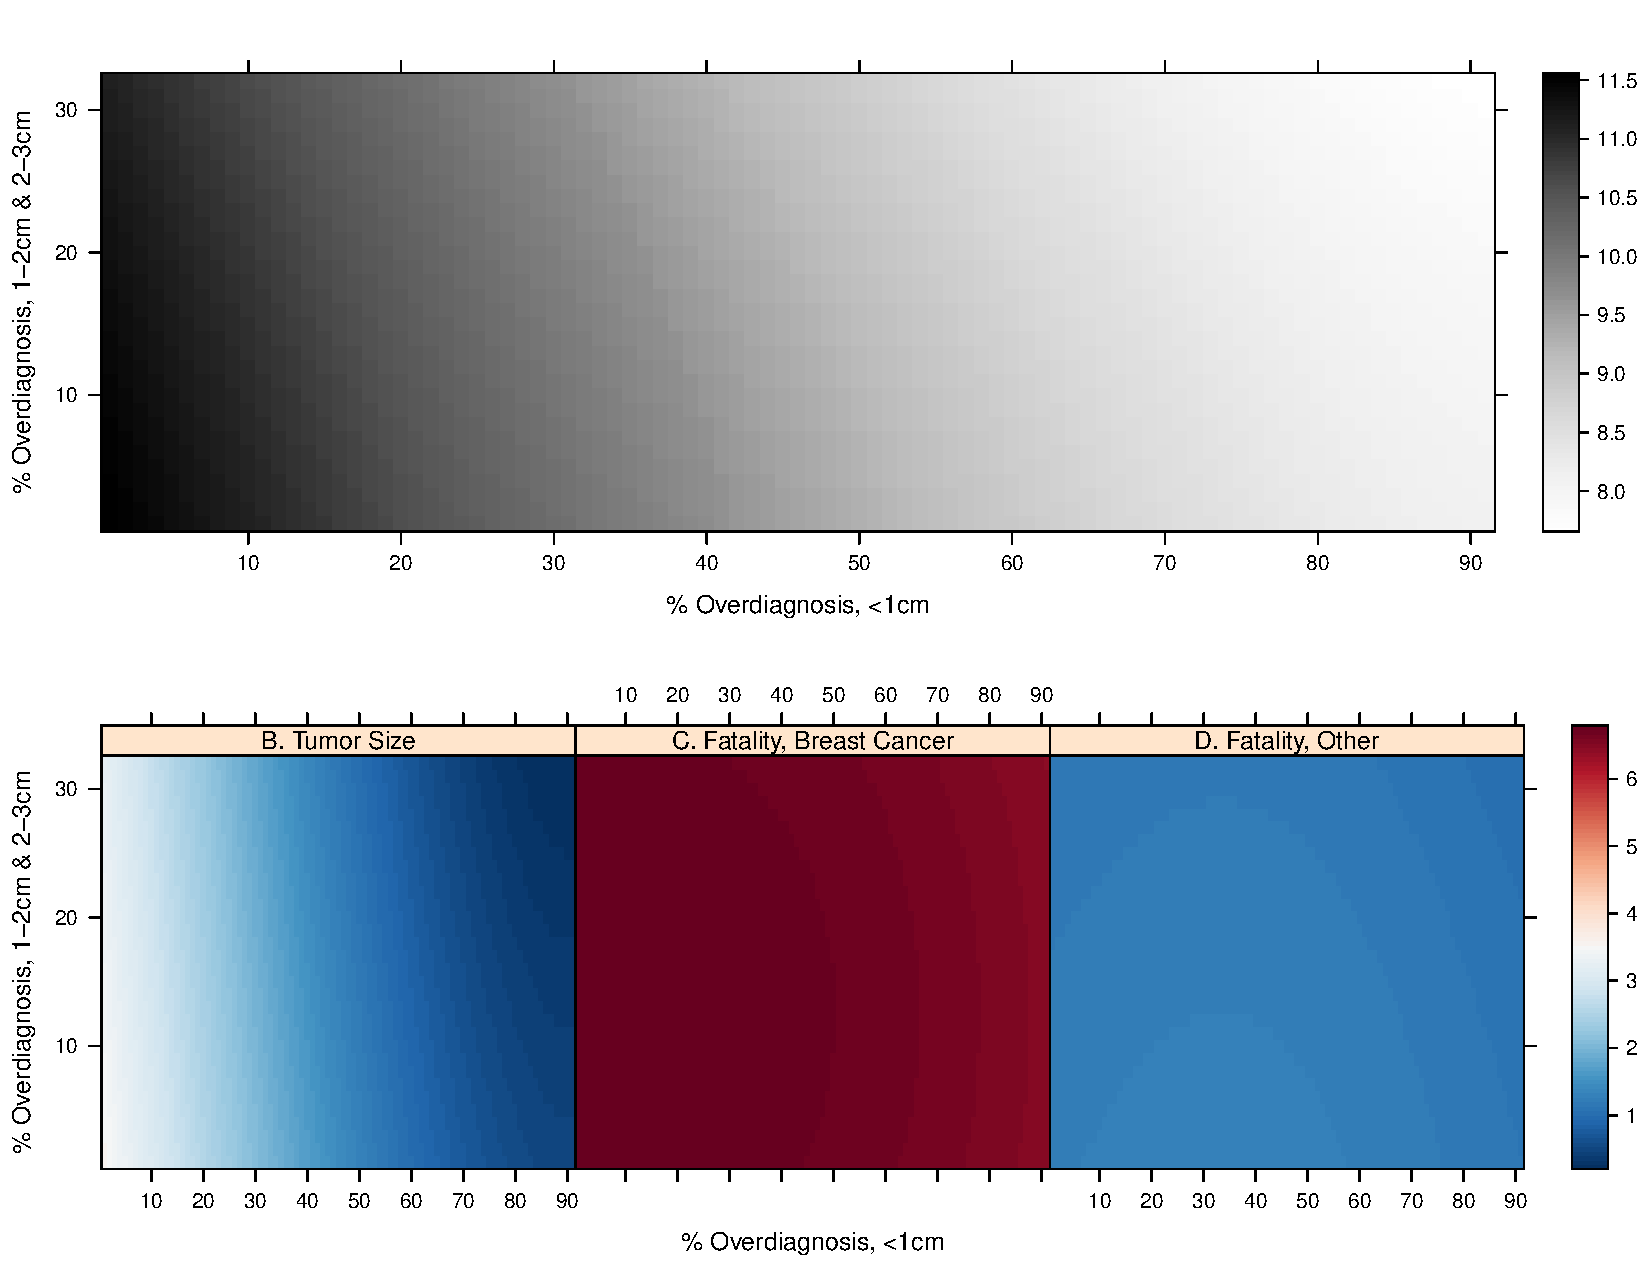
\includegraphics[width=\linewidth]{appendix_figure2}
\spacingset{1}\caption{Gain in life expectancy (top panel) and
  contributions of the temporal shift to smaller sized tumors (bottom
  left), temporal reductions in case fatality rates from breast cancer
  (bottom center), and temporal reductions in case fatality rates from
  competing causes of death (bottom right) varying the overdiagnosis
  level for $<1$cm tumors (0\% to 90\%) and 1-3cm tumors (0\% to
  31\%).  The color scale for the top (bottom) panel indicates the
number of years of the gain in life expectancy (contribution to the gain).}
\label{fig:figure2}
\end{center}
\end{figure}

\newpage
\section{Varying Time Intervals Between Diagnosis and Death}
\spacingset{1}

\begin{center}
  \begin{table}[h]
\begin{tabular}{@{}l rrrr@{}}
  Time & Gain in Life & &
                                \multicolumn{2}{c}{\underline{Reductions
                                in Case Fatality Rates from}}\\
  Interval & Expectancy & Tumor Size  & Breast Cancer   & Competing Causes  \\ 
  \midrule
  8  & 11.23 & 3.15 (28\%) & 7.07 (63\%) & 1.03 (9\%) \\ 
  9  & 10.93 & 3.09 (28\%) & 6.76 (62\%) & 1.09 (10\%) \\ 
  10  & 10.69 & 2.99 (28\%) & 6.57 (61\%) & 1.15 (11\%) \\ 
  11  & 10.38 & 2.78 (27\%) & 6.27 (60\%) & 1.35 (13\%) \\ 
  12  & 10.28 & 2.65 (26\%) & 6.05 (59\%) & 1.59 (15\%) \\ 
  \bottomrule
\end{tabular}
\caption{Gain in life expectancy and contribution of the temporal shift to smaller sized tumors, temporal reductions in case fatality rates from breast cancer, and temporal reductions in case fatality rates from
  competing causes of death, 1975-2000, varying time interval between breast
  cancer diagnosis and death.  Note: Yrs=years.}
\end{table}
\end{center}

\newpage
\spacingset{1} \pdfbookmark[1]{References}{References}
\bibliography{cancer}
\end{document}



